\chapter{Supplementary Material of Chapter \ref{chap:pinn-bo}} 
\label{section:pinn-bo_supp}
\section{Additional Experimental Results}
\subsection{Synthetic Benchmark Functions}
\label{section:pinn-bo_experiments_synthetic}
We present the mathematical expressions of five synthetic objective functions and their accompanied PDEs used in Section 5 of the main paper as follows: 
\paragraph{Drop-Wave:} 
\begin{align*}
    f(\mathbf{x}) &= - \frac{1 + \cos(12\sqrt{\mathbf{x}_1^2 + \mathbf{x}_2^2})}{0.5(\mathbf{x}_1^2 + \mathbf{x}_1^2) + 2} \text{ s.t. } \mathbf{x}_1 \frac{\partial f}{\partial \mathbf{x}_2} - \mathbf{x}_2 \frac{\partial f}{\partial \mathbf{x}_1} = 0
\end{align*}
\paragraph{Styblinski-Tang:}
\begin{align*}
        f(\mathbf{x}) &= \frac{1}{2} \sum_{i=1}^{d} (\mathbf{x}_i^4 - 16\mathbf{x}_i^2 + 5\mathbf{x}_i) \text{ s.t. }  \sum_{i=1}^d \frac{\partial f}{\partial \mathbf{x}_i} = \sum_{i=1}^{d}(2\mathbf{x}_i^3 -16\mathbf{x}_i +\frac{5}{2})
\end{align*}

\paragraph{Rastrigin:}
\begin{align*}
        f(\mathbf{x}) &= 10d + \sum_{i=1}^{d} \left[ \mathbf{x}_i^2 - 10 \cos(2\pi \mathbf{x}_i) \right] 
        \\
        \text{s.t. }  &\mathbf{x}^\top \nabla f(\mathbf{x})  - f(\mathbf{x}) = 10\sum_{i=1}^d \left[ (\cos(2\pi \mathbf{x}_i)) + \pi \mathbf{x}_i (\sin(2\pi \mathbf{x}_i)) - 1 \right]
\end{align*}
\paragraph{Michalewics:}
\begin{align*}
        f(\mathbf{x}) &= -\sum_{i=1}^{d} \sin(\mathbf{x}_i) \sin^{2m}\left(\frac{i\mathbf{x}_i^2}{\pi}\right) \text{ s.t. } \mathbf{h}^\top \nabla f(\mathbf{x}) - f(\mathbf{x}) = 0,\\ & \text{where } \mathbf{h} = [\mathbf{h}_1, \mathbf{h}_2, \dots, \mathbf{h}_d]^\top, \mathbf{h}_i = \left[\frac{\cos(\mathbf{x}_i)}{\sin(\mathbf{x}_i)} + \frac{2\mathbf{x}_i (2m-1)}{\tan(\frac{i\mathbf{x}_i^2}{\pi})}\right]^{-1}
\end{align*}
\paragraph{Cosine Mixture:}
\begin{align*}
    0.1 \sum_{i=1}^d \cos(5\pi\mathbf{x}_i) + \sum_{i=1}^d \mathbf{x}_i^2 \text{ s.t } \sum_{i=1}^d \left(\frac{\partial f}{\partial \mathbf{x}_i} - 2\mathbf{x}_i + 0.5\pi\sin(5\pi\mathbf{x}_i) \right)^2 = 0
\end{align*}

% \subsection{Real-world Applications}
% \label{section:pinn-bo_experiments_real_world}
% \subsubsection{Optimizing Steady-State Temperature}
% \label{section:pinn-bo_experiments_2d_laplace}
% In this study, we showcase the benchmark optimization outcomes achieved by our proposed PINN-BO algorithm, comparing them with baseline methods for the steady-state temperature optimization task.  The governing PDE dictating the temperature distribution is expressed as: $\nabla^2 T(x, y) = 0$. We explore the heat equation in a domain where $x$ and $y$ lie within the defined range of $[0,2\pi]$. To thoroughly investigate the problem, we consider three distinct boundary conditions for this equation, each contributing to a nuanced understanding of the system: 

%  \paragraph{Heat Equation with boundary conditions 1}
%  \label{para:heat1}
%  \begin{align*}
%      T(x, 0) &= 5\sin(y) + \sqrt{1+y} \\
%     T(x, 2\pi) &= y\sin\left(3\cos(y) + 2\exp(y)\sin(y)\right) \\
%    T(0, y) &= 10\cos(x) + x\exp(\sqrt{x^2 + \sin(x)}) \\
%    T(2\pi, y) &= 3\sqrt{\exp(x\exp(-x))}\sin(x) + \cos(3x)\cos(3x)
%  \end{align*}
%  \paragraph{Heat Equation with boundary conditions 2}
%  \label{para:heat2}
% \begin{align*}
%     T(x, 0) &= \sin(x) \cos(2x) + x^2\sqrt{3x}  + e^{\sin(x)} \\
%     T(x, 2\pi) &= e^{\sin(x)} \sqrt{3x} + x^2 \cos(x)  \sin^2(x)   + e^{\cos(x)} \\
%     T(0, y) &= \sqrt{2y}  \sin(y) + y^3\cos(2y)   + e^{\cos(y)} \\
%     T(2\pi, y) &= \sin(y) \cos(2y) + y^3\sqrt{2y}   + e^{\sin(y)}
% \end{align*}
% \paragraph{Heat Equation with boundary conditions 3}
% \label{para:heat3}
% \begin{align*}
%     T(x, 0) &= \left(\sin(x) + \cos(2x) \right) \sqrt{3x} + x^2 + e^{\sin(x)} \\
%     T(x, 2\pi) &= \left(e^{\sin(x)} + \sqrt{3x} \right) \cos(x) + \left(\sin^2(x) + x^2\right)  e^{\cos(x)}
%     \\
%     T(0, y) &= \left(\sqrt{2y} + \sin(y)\right)  \left(\cos(2y) + y^3 \right) + e^{\cos(y)}\\
%     T(2\pi, y) &= \left(\sin(y) + \cos(2y)\right) \left(\sqrt{2y} + y^3\right) + e^{\sin(y)}
% \end{align*}
% We utilized py-pde, a Python package designed for solving partial differential equations (PDEs), available at the following GitHub repository: \url{https://github.com/zwicker-group/py-pde}. This tool enabled us to obtain solutions to heat equations at various input points, with specific boundary conditions serving as the input data. In Figure \ref{fig:heat_dist}, the temperature distribution within the defined domain $[0, 2\pi]$ is visualized. It is important to emphasize that the boundary conditions used for benchmarking purposes are unknown to the methods employed. Adhering to the framework of black-box optimization, we assume that solving the PDEs incurs a substantial computational cost. The figure illustrates the spatial distribution of temperature values $T(x,y)$ across domain $[0, 2\pi] \times [0, 2\pi]$, with each subfigure corresponding to one of the aforementioned boundary conditions. 
% \begin{figure}[ht]
%     \centering
%     \begin{subfigure}[b]{0.3\textwidth}
%         \centering
%         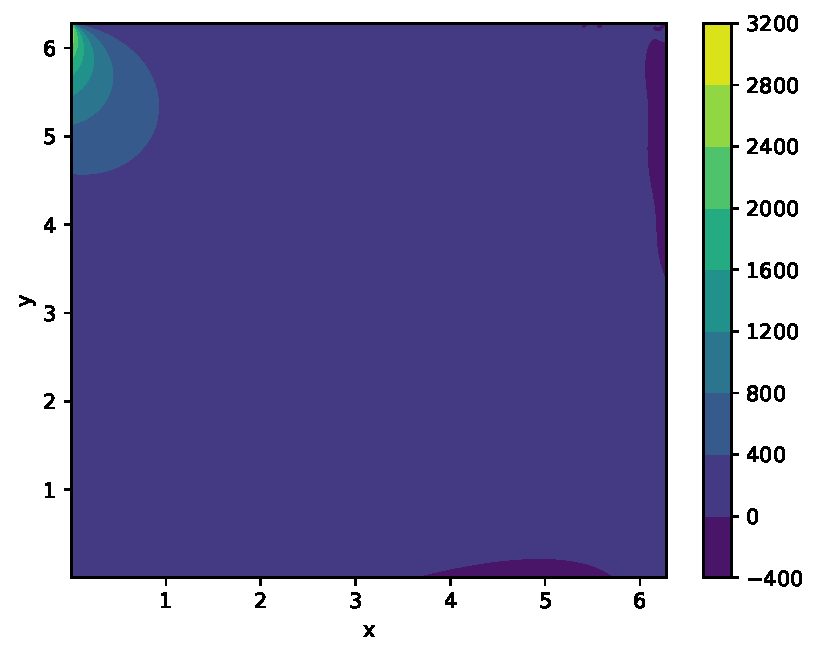
\includegraphics[width=\textwidth]{Figures/PINN-BO/heat_py_pde_1000_test_1.pdf}
%         \caption{Solution of Temperature Equation with boundary conditions 1}
%  \label{fig:heat_1_dist}
%     \end{subfigure}
%     \hfill
%     \begin{subfigure}[b]{0.3\textwidth}
%         \centering
%         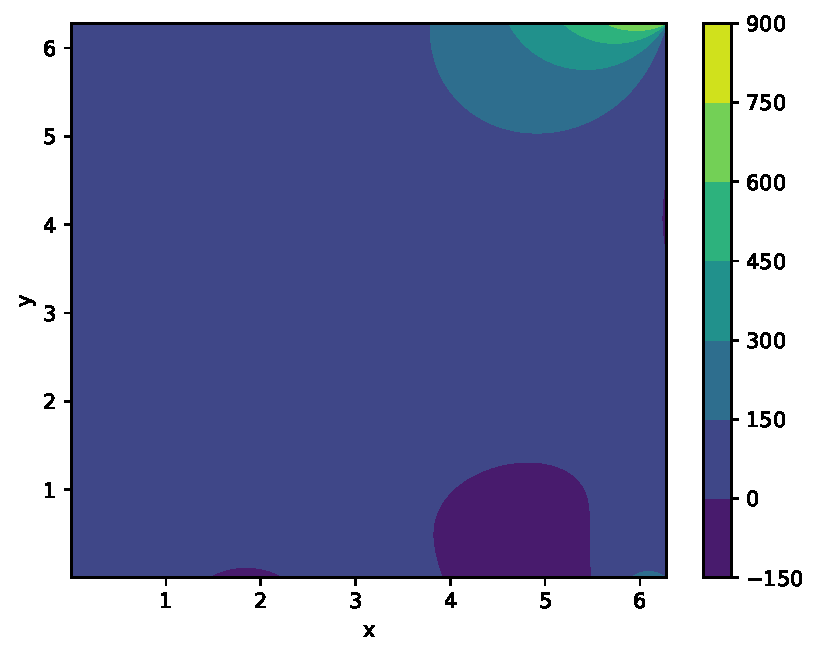
\includegraphics[width=1\textwidth]{Figures/PINN-BO/heat_py_pde_1000_test_2.pdf}
%         \caption{Solution of Temperature Equation with boundary conditions 2}
%         \label{fig:heat_2_dist}
%     \end{subfigure}
%     \hfill
%     \begin{subfigure}[b]{0.3\textwidth}
%         \centering
%         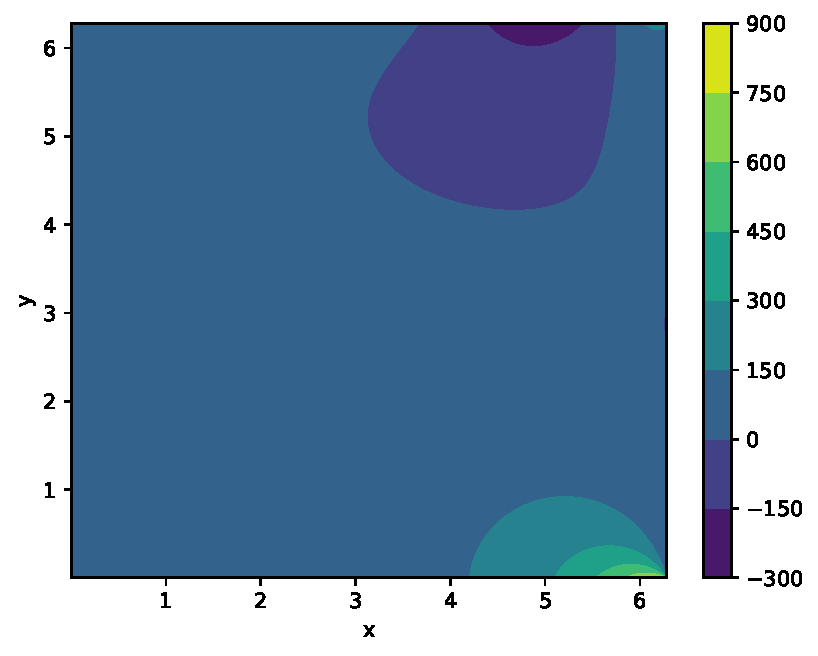
\includegraphics[width=\textwidth]{Figures/PINN-BO/heat_py_pde_1000_test_3.pdf}
%         \caption{Solution of Temperature Equation with boundary conditions 3}
%         \label{fig:heat_3_dist}
%     \end{subfigure}
%     \caption{The figures depict the solutions for temperature distributions governed by the heat equation, with each figure corresponding to a specific tuple of boundary conditions described in Section \ref{section:pinn-bo_experiments_2d_laplace}. It is evident that the region with the highest temperature is relatively small in comparison to the entire domain.}
%     \label{fig:heat_dist}
% \end{figure}

% We conducted temperature optimization by identifying the locations $(x,y)$ where the temperature reaches its maximum. As illustrated in Figure \ref{fig:heat_dist}, the area with high temperatures is relatively small in comparison to the regions with medium or low temperatures. For each baseline, we performed the optimization process 10 times, computing the average results. The comparative outcomes are presented in Figure \ref{fig:heat_opt}. 
% \begin{figure}[ht]
%     \centering
%     \begin{subfigure}[b]{0.3\textwidth}
%         \centering
%     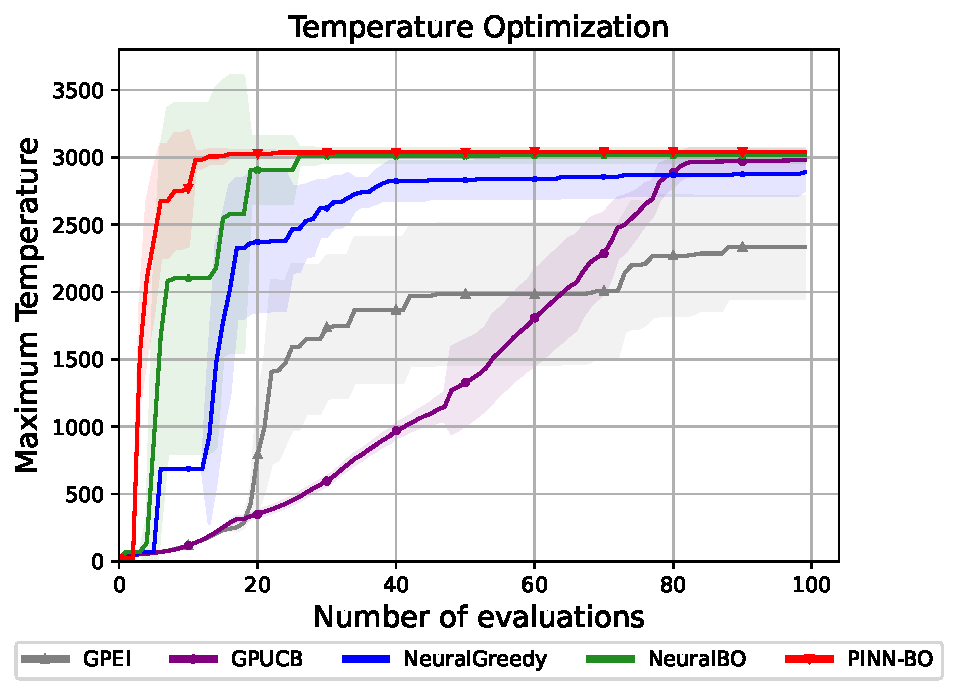
\includegraphics[width=\textwidth]{Figures/PINN-BO/Heat_dim_2_bc1.pdf}
%         \caption{Temperature Optimization in case of boundary conditions 1}
%  \label{fig:heat_1_opt}
%     \end{subfigure}
%     \hfill
%     \begin{subfigure}[b]{0.3\textwidth}
%         \centering
%         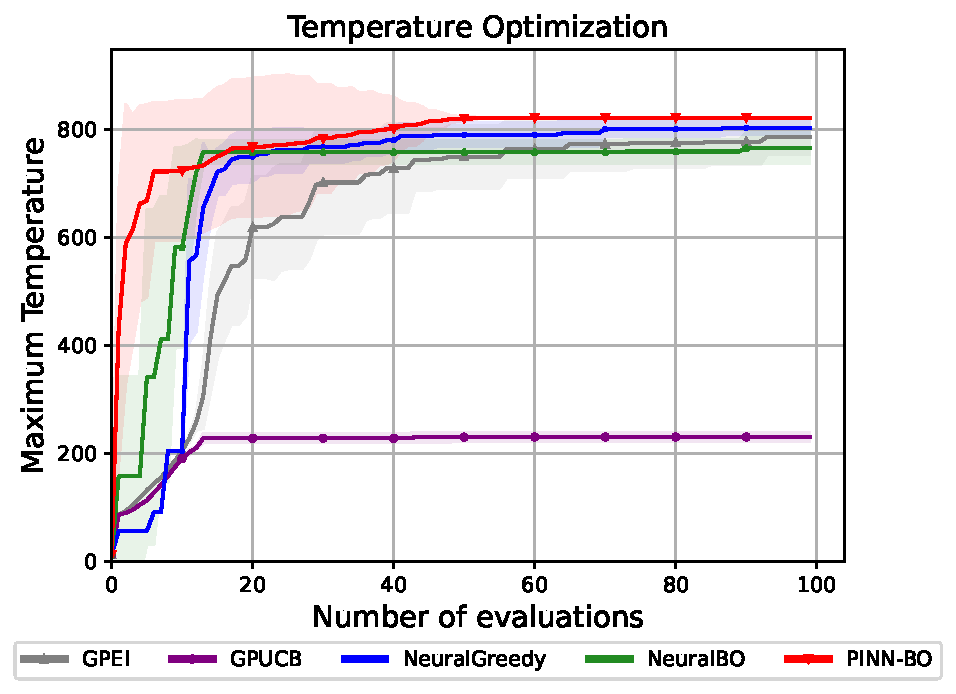
\includegraphics[width=1\textwidth]{Figures/PINN-BO/Heat_dim_2_bc2.pdf}
%         \caption{Temperature Optimization in case of boundary conditions 2}
%         \label{fig:heat_2_opt}
%     \end{subfigure}
%     \hfill
%     \begin{subfigure}[b]{0.3\textwidth}
%         \centering
%         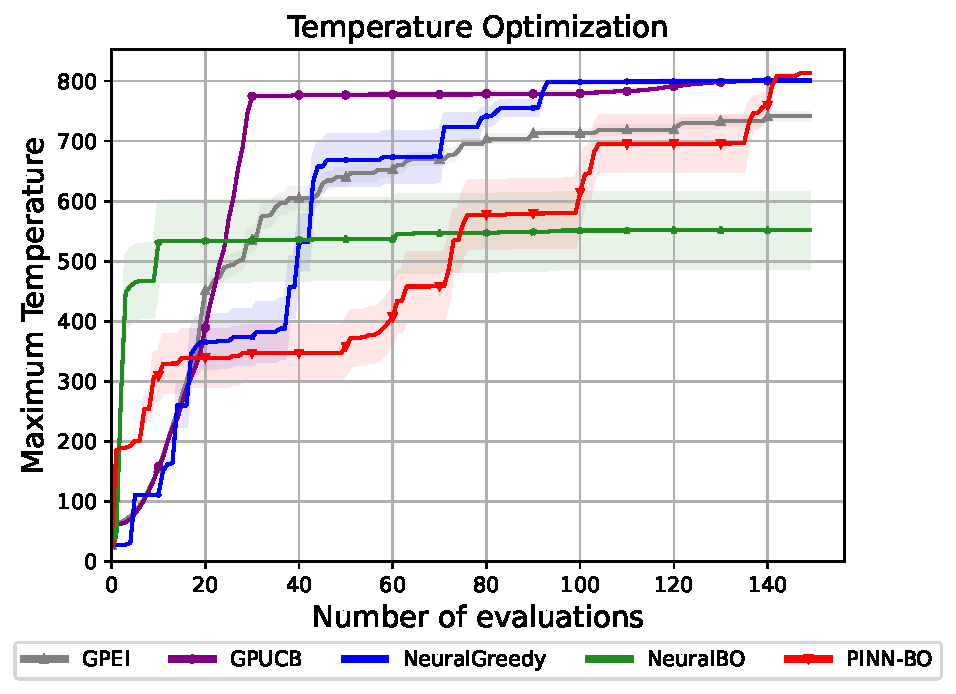
\includegraphics[width=\textwidth]{Figures/PINN-BO/Heat_dim_2_bc3.pdf}
%         \caption{Temperature Optimization in case of boundary conditions 3}
%         \label{fig:heat_3_opt}
%     \end{subfigure}
%     \caption{The figure shows the temperature optimization results of our PINN-BO and other baselines. For all three cases with different positions of maximum temperature, our PINN-BO performs better than all other baselines.}
%     \label{fig:heat_opt}
% \end{figure}


% \subsubsection{Optimizing Beam Displacement}
% We showcase the benchmark optimization outcomes obtained through our proposed method, PINN-BO, and the baseline approaches, addressing the task of minimizing the deflection of a non-uniform Euler-Bernoulli beam. The governing differential equation describing the behavior of a non-uniform Euler-Bernoulli beam is provided below: 
% \begin{equation*}
%     \frac{d^2}{dx^2} \left( EI(x) \frac{d^2 w(x)}{dx^2} \right) = q(x),
% \end{equation*}
% where
% $EI(x)$ represents the flexural rigidity of the beam, which can vary with position $x$, and $w(x)$ represents the vertical displacement of the beam at position $x$ and 
% $q(x)$ represents the distributed or concentrated load applied to the beam. 
% In our implementation, we consider the detailed expression of $EI(x)$ and $q(x)$ as follows:
% \begin{align*}
%     EI(x) &= \frac{e^x}{\rho(x)},\\
%     \rho(x) &= 2.4 x - 64 \pi^{2} e^{4 x} \sin{\left(4 \pi e^{2 x} \right)} - 396 e^{2 x} \sin{\left(20 x \right)} \\
%     &+ 80 e^{2 x} \cos{\left(20 x \right)} + 16 \pi e^{2 x} \cos{\left(4 \pi e^{2 x} \right)} + 0.4
% \end{align*}
% We employed the Finite Difference Method (FDM) to solve the non-uniform Euler-Bernoulli beam equation. It's crucial to note that this step is solely for generating observations at each input point. Despite obtaining this solution, our methods and all baseline techniques continue to treat this solution as a black-box function, accessing observations solely through querying. In Figure \ref{fig:beam_illustration}, the displacement values $w(x)$ for $x \in (0,1)$ are illustrated. The optimization results for both our PINN-BO and the other baseline methods are presented in Figure \ref{fig:beam_opt}.

% \begin{figure}[ht]
%     \centering
%     \begin{subfigure}[b]{0.44\textwidth}
%         \centering
%     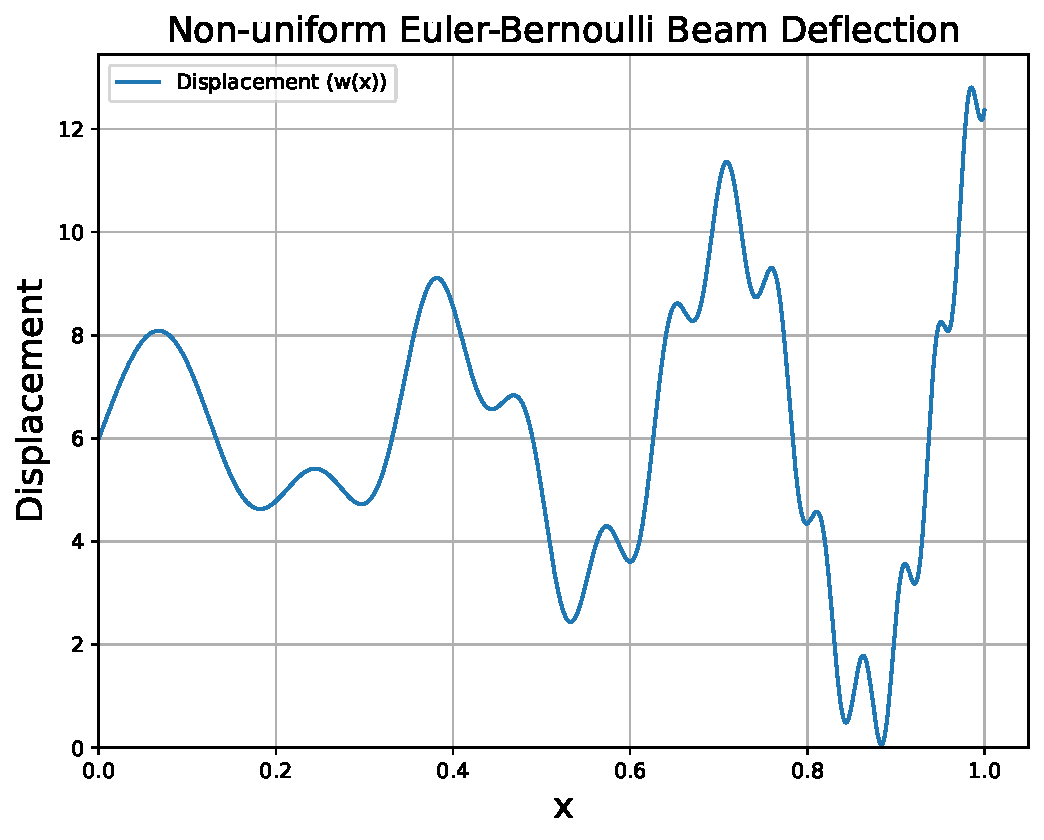
\includegraphics[width=\textwidth]{Figures/PINN-BO/beam.pdf}
%     \caption{Displacement of non-uniform Euler beam}
%      \label{fig:beam_illustration}
%     \end{subfigure}
%     \hfill
%     \begin{subfigure}[b]{0.49\textwidth}
%         \centering
%         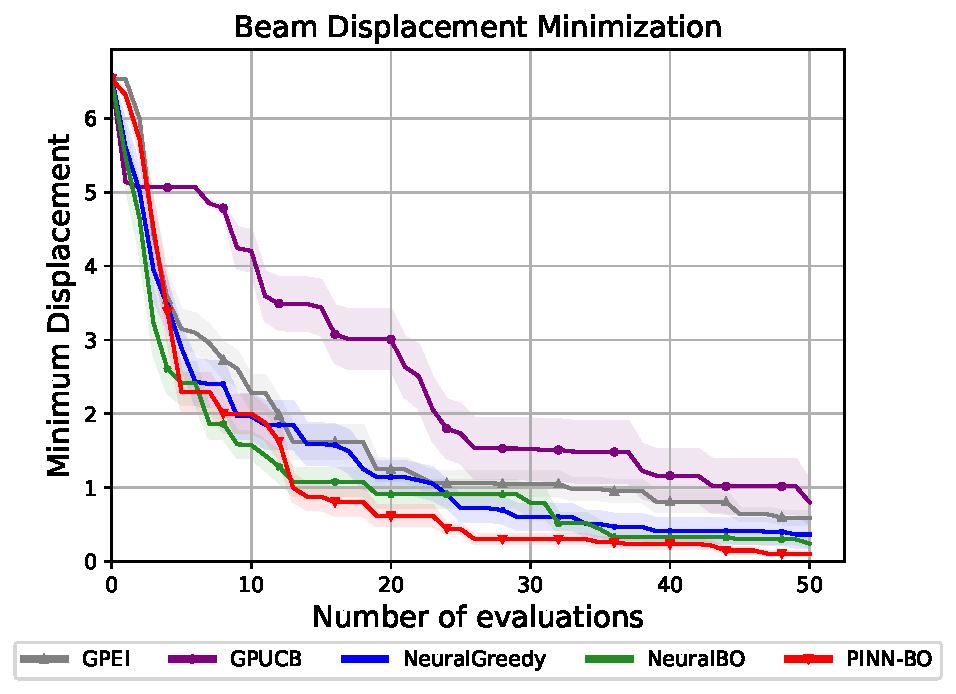
\includegraphics[width=1\textwidth]{Figures/PINN-BO/BeamDeflection_dim_1.pdf}
%         \caption{Displacement Optimization of non-uniform Euler beam}
%         \label{fig:beam_opt}
%     \end{subfigure}
%     \caption{Displacement of a Non-uniform Euler Beam and minimum displacement found by our PINN-BO and the other baselines. The left panel illustrates the natural displacement profile of the non-uniform Euler beam under given loads $q(x)$,  flexural rigidity $EI(x)$, and boundary conditions. The right panel depicts the optimized position on the beam where the displacement is minimized, highlighting the location where the structural response is at its lowest. }
%     \label{fig:beam}
% \end{figure}
\section{Proof of Theoretical Analysis in Chapter \ref{chap:pinn-bo}}
\label{section:pinn-bo_appendix}

\subsection{Proof of Lemma \ref{lemma:pinn-bo_PINN_mean_cov}}
In this section, we present the detailed proof of Lemma \ref{lemma:pinn-bo_PINN_mean_cov} in the main paper. Before going to the proof, we repeat Lemma \ref{lemma:pinn-bo_PINN_mean_cov} here:
\PinnMeanCov*

\textbf{To prove Lemma \ref{lemma:pinn-bo_PINN_mean_cov}, we need the following lemma:}

\begin{lemma}{(Theorem 4.1 \citet{wang2022and})}
\label{lemma:PINN_GP}
A sufficiently wide physics-informed neural network for modeling the problem defined in Section 4 induces a joint multivariate
Gaussian distribution between the network outputs and its ``derivatives'' after applying the differential operator to this network
\begin{align}
    \begin{bmatrix}
        \mathbf{h}_{\boldsymbol{\theta}} \\
        \mathbf{g}_{\boldsymbol{\theta}} 
\end{bmatrix} \sim N(\mathbf{0}, \mathbf{K}_\mathrm{NTK-PINN}),
\end{align} 
where $\mathbf{K}_\mathrm{NTK-PINN} = \begin{bmatrix}
    \mathbf{K}_{uu} & \mathbf{K}_{ur} \\
    \mathbf{K}_{ru} & \mathbf{K}_{rr}
\end{bmatrix}$ is the NTK matrix of PINN, with
\begin{align}
    (\mathbf{K}_{uu})_{ij} &= \langle \phi(\mathbf{x}_i), \phi(\mathbf{x}_j) \rangle \\ 
    (\mathbf{K}_{ur})_{ij} &= \langle \phi(\mathbf{x}_i), \omega(\mathbf{z}_j) \rangle
    \\
    (\mathbf{K}_{uu})_{ij} &= \langle \omega(\mathbf{z}_i), \omega(\mathbf{z}_j) \rangle
    \\
    \mathbf{K}_{ru} &= \mathbf{K}_{ur}^\top, \\ 
    \mathbf{h}_{\boldsymbol{\theta}} &= [h(\mathbf{x}_1, \boldsymbol{\theta}), \dots, h(\mathbf{x}_t, \boldsymbol{\theta})]^\top
    \\
    \mathbf{g}_{\boldsymbol{\theta}} &= \left[\mathcal{N}[h](\mathbf{z}_1, \boldsymbol{\theta}), \dots, \mathcal{N}[h](\mathbf{z}_{N_r}, \boldsymbol{\theta}) \right]^\top
\end{align}
where $\mathbf{x}_i, \mathbf{x}_j \in \mathcal{D}_t$ and $\mathbf{z}_i, \mathbf{z}_j \in \mathcal{R}$ are two arbitrary points belonging to the set $\mathcal{R}$ defined in Algorithm 1 and $\mathcal{N}[h]$ denotes a differential operator of the neural network $h(\cdot, \boldsymbol{\theta})$ with respect to the input $\mathbf{x}$. 
\end{lemma}
\begin{subcorollary}
\label{corollary:pinn-bo_PINN_GP_func}
    The unknown reward function values $f_{1:t}$ and the PDE observations $g_{1:N_r}$ are jointly Gaussian with an initial prior distribution with zero mean and the covariance $\nu_t^2 \mathbf{K}_\mathrm{NTK-PINN}$, where $\nu_t$ is the exploration coefficient introduced in Section 4. 
    \begin{align}
    \begin{bmatrix}
        f_{1:t} \\
        g_{1:N_r}
\end{bmatrix} \sim N(\mathbf{0}, \nu_t^2 \mathbf{K}_\mathrm{NTK-PINN}),
\end{align} 
\end{subcorollary}

\begin{proof}[Proof of Corollary  \ref{corollary:pinn-bo_PINN_GP_func}]
The algorithm updates the neural network by minimizing the loss function: \begin{equation}
    \mathcal{L}(t) = \sum^{t-1}_{i=1} [y_i - \nu_t h(\mathbf{x}_i; \boldsymbol{\theta}_{t-1})]^2 + \sum^{N_r}_{j=1}[u_j - \nu_t \mathcal{N}[h](\mathbf{z}_j; \boldsymbol{\theta}_{t-1})]^2
\end{equation} 
As the function prediction and its ``derivatives" prediction of each observation $\mathbf{x}_i$ and $\mathbf{z}_j$ at iteration $t$ is modeled by $\nu_t h(\mathbf{x}_i; \boldsymbol{\theta}_{t-1})$ and $\nu_t \mathcal{N}[h](\mathbf{z}_j; \boldsymbol{\theta}_{t-1})$, it is clear to see, from Lemma \ref{lemma:PINN_GP}, that the function values of the unknown function $f$ can be assumed to follow a joint Gaussian prior with zero means and covariance matrix $\nu_t^2 \mathbf{K}_\mathrm{NTK-PINN}$. A similar argument can be applied to the function $g$, where $g(\cdot) = \mathcal{N}[f] (\cdot)$ with $\mathcal{N}[f]$ is a differential operator. We are now ready to prove \ref{lemma:pinn-bo_PINN_mean_cov}.
\end{proof} 
\begin{proof} [Proof of Lemma \ref{lemma:pinn-bo_PINN_mean_cov}]
From Corollary \ref{corollary:pinn-bo_PINN_GP_func}, the priors for values of both $f$ and $g$ follow a joint Gaussian distribution with kernel $\mathbf{K}_\mathrm{NTK-PINN}$. Let $\mathbf{K_x}$ be the NTK matrix between point $\mathbf{x}$ and all training data: $\mathbf{K}_x = \begin{bmatrix}
        \Sigma_a & \Sigma_b \\
        \Sigma_c & \Sigma_d
    \end{bmatrix} =\begin{bmatrix}
         \boldsymbol{\Phi}_t \phi(\mathbf{x}) & 
         \boldsymbol{\Phi}_t \omega(\mathbf{x}) \\
         \boldsymbol{\Omega}_r\phi(\mathbf{x}) &
          \boldsymbol{\Omega}_r  \omega(\mathbf{x})  \end{bmatrix}$. 
Then the the posterior of $f$ and $g$ evaluated at an input $\mathbf{x}$ will be a Gaussian distribution with mean and variance functions:
\paragraph{Mean function:}
\begin{align*}
    &\;\;\;\; \begin{bmatrix}
        \mu_t^f(\mathbf{x})\\
        \mu_t^g(\mathbf{x}) 
    \end{bmatrix} = \mathbf{K}_\mathbf{x} ^\top \mathbf{\widehat{K}}_\mathrm{PINN}^{-1} \begin{bmatrix}
        \mathbf{Y}_t \\
        \mathbf{U}_r
    \end{bmatrix}
    \\
    &= \begin{bmatrix}
        \Sigma_a^\top & \Sigma_c^\top \\
        \Sigma_b^\top & \Sigma_d^\top
    \end{bmatrix} \begin{bmatrix}
        \widetilde{\mathbf{A}} & \widetilde{\mathbf{B}} \\
    \widetilde{\mathbf{C}} & \widetilde{\mathbf{D}}
    \end{bmatrix} \begin{bmatrix}
        \mathbf{Y}_t \\
        \mathbf{U}_r
    \end{bmatrix}\\
    &= \begin{bmatrix}
        \phi(\mathbf{x})^\top \boldsymbol{\Phi}_t^\top &  \phi(\mathbf{x})^\top \boldsymbol{\Omega}_r ^\top \\
        \omega(\mathbf{x})^\top \boldsymbol{\Phi}_t^\top  & \omega(\mathbf{x})^\top \boldsymbol{\Omega}_r ^\top
    \end{bmatrix} \begin{bmatrix}
        \widetilde{\mathbf{A}} & \widetilde{\mathbf{B}} \\
    \widetilde{\mathbf{C}} & \widetilde{\mathbf{D}}
    \end{bmatrix} \begin{bmatrix}
        \mathbf{Y}_t \\
        \mathbf{U}_r
    \end{bmatrix} \\
    & = \begin{bmatrix}
         \phi(\mathbf{x})^\top \boldsymbol{\Phi}_t^\top \widetilde{\mathbf{A}}\mathbf{Y}_t +  \phi(\mathbf{x})^\top \boldsymbol{\Omega}_r ^\top  \widetilde{\mathbf{C}}\mathbf{Y}_t  + \phi(\mathbf{x})^\top \boldsymbol{\Phi}_t^\top \widetilde{\mathbf{B}} \mathbf{U}_r   +  \phi(\mathbf{x})^\top \boldsymbol{\Omega}_r ^\top  \widetilde{\mathbf{D}} \mathbf{U}_r \\
         \omega(\mathbf{x})^\top \boldsymbol{\Phi}_t^\top \widetilde{\mathbf{A}} \mathbf{Y}_t +  \omega(\mathbf{x})^\top \boldsymbol{\Omega}_r ^\top  \widetilde{\mathbf{C}} \mathbf{Y}_t  +\omega(\mathbf{x})^\top \boldsymbol{\Phi}_t^\top \widetilde{\mathbf{B}} \mathbf{U}_r  +  \omega(\mathbf{x})^\top \boldsymbol{\Omega}_r ^\top  \widetilde{\mathbf{D}} \mathbf{U}_r
    \end{bmatrix}
        \\
         &=\phi(\mathbf{x})^\top \boldsymbol{\xi}_t^\top \mathbf{\widehat{K}}_\mathrm{PINN}^{-1} \begin{bmatrix}
         \mathbf{Y}_t \\
         \mathbf{U}_r\end{bmatrix}
\end{align*}

\paragraph{Variance function:}
Let $\mathbf{K}_{\mathbf{xx}} = \begin{bmatrix}
\langle \phi(\mathbf{x}), \phi(\mathbf{x}) \rangle & \langle \phi(\mathbf{x}), \omega(\mathbf{x}) \rangle \\
\langle \omega(\mathbf{x}), \phi(\mathbf{x}) \rangle & \langle \omega(\mathbf{x}), \omega(\mathbf{x}) \rangle
\end{bmatrix}$, then we have the posterior covariance matrix of $f$ and $g$ at input $\mathbf{x}$ is:
\begin{align}
    &\begin{bmatrix}
    \mathrm{Cov}_f(\mathbf{x}) & \mathrm{Cov}_{fg}(\mathbf{x}) \\
    \mathrm{Cov}_{gf}(\mathbf{x}) & \mathrm{Cov}_g(\mathbf{x})
\end{bmatrix}  \\
&= \nu_t^2 \left(\mathbf{K}_{\mathbf{xx}} - \mathbf{K_x}^\top \mathbf{\widehat{K}}_\mathrm{PINN}^{-1} \mathbf{K_x} \right) \\
&= \nu_t^2   \begin{bmatrix}
\langle \phi(\mathbf{x}), \phi(\mathbf{x}) \rangle & \langle \phi(\mathbf{x}), \omega(\mathbf{x}) \rangle \notag \\
\langle \omega(\mathbf{x}), \phi(\mathbf{x}) \rangle & \langle \omega(\mathbf{x}), \omega(\mathbf{x}) \rangle
\end{bmatrix} - \nu_t^2
\begin{bmatrix}
        \Sigma_a^\top& \Sigma_c^\top \\
        \Sigma_b^\top & \Sigma_d^\top
\end{bmatrix} \begin{bmatrix}
    \widetilde{\mathbf{A}} & \widetilde{\mathbf{B}} \\
    \widetilde{\mathbf{C}} & \widetilde{\mathbf{D}}
        \end{bmatrix}  \begin{bmatrix}
                            \Sigma_a & \Sigma_b \\
                            \Sigma_c & \Sigma_d
                        \end{bmatrix}  \\
\end{align}
Therefore, 
\begin{align}
\mathrm{Cov}_f(\mathbf{x}) & = \nu_t^2 \langle \phi(\mathbf{x}),  \phi(\mathbf{x}) \rangle - \nu_t^2(\Sigma_a^\top \widetilde{\mathbf{A}}\Sigma_a + \Sigma_c^\top \widetilde{\mathbf{C}}\Sigma_c + \Sigma_a^\top \widetilde{\mathbf{B}}\Sigma_a + \Sigma_c^\top \widetilde{\mathbf{D}}\Sigma_c) \\
        & = \nu_t^2 \langle \phi(\mathbf{x}),  \phi(\mathbf{x}) \rangle - \nu_t^2 \begin{bmatrix}
            \Sigma_a^\top  & \Sigma_c^\top
        \end{bmatrix}
        \begin{bmatrix}
    \widetilde{\mathbf{A}} & \widetilde{\mathbf{B}} \\
    \widetilde{\mathbf{C}} & \widetilde{\mathbf{D}}
        \end{bmatrix} \begin{bmatrix}
            \Sigma_a \\ \Sigma_c
        \end{bmatrix}  \\
        &= \nu_t^2 \langle \phi(\mathbf{x}),  \phi(\mathbf{x}) \rangle - \nu_t^2\begin{bmatrix}
            \phi(\mathbf{x})^\top \boldsymbol{\Phi}_t^\top & \phi(\mathbf{x})^\top \boldsymbol{\Omega}_r^\top
        \end{bmatrix}  \begin{bmatrix}
    \widetilde{\mathbf{A}} & \widetilde{\mathbf{B}} \\
    \widetilde{\mathbf{C}} & \widetilde{\mathbf{D}}
        \end{bmatrix} \begin{bmatrix} \boldsymbol{\Phi}_t \phi(\mathbf{x}) \\ \boldsymbol{\Omega}_r \phi(\mathbf{x})  \end{bmatrix}  \\
        &= \nu_t^2 \langle \phi(\mathbf{x}),  \phi(\mathbf{x}) \rangle - \nu_t^2\phi(\mathbf{x})^\top \boldsymbol{\xi}_t^\top \mathbf{\widehat{K}}_\mathrm{PINN}^{-1} \boldsymbol{\xi}_t \phi(\mathbf{x})\\
        &= \nu_t^2 (\sigma_t^f)^2(\mathbf{x})
\end{align}
\end{proof}
\subsection{Proof of Lemma \ref{lemma:interaction_information_formula}}
\begin{lemma}
    \label{lemma:interaction_information_formula}
    The interaction information between $f$ and observation $\mathbf{Y}_t$ and PDE data $\mathbf{U}_r$, for the points chosen from Algorithm 1 can be calculated as:
    \begin{equation*}
        I (f; \mathbf{Y}_t; \mathbf{U}_r) = \frac{1}{2}  \log (\frac{\det(\frac{\boldsymbol{\Phi}_t^\top \boldsymbol{\Phi}_t}{\lambda_1} + \mathbf{I})\det(\frac{\boldsymbol{\Omega}_r^\top \boldsymbol{\Omega}_r}{\lambda_2} + \mathbf{I})}{\det(\frac{\boldsymbol{\Phi}_t^\top \boldsymbol{\Phi}_t}{\lambda_1} + \frac{\boldsymbol{\Omega}_r^\top \boldsymbol{\Omega}_r}{\lambda_2} + \mathbf{I})})
    \end{equation*}
\end{lemma}
\textbf{To prove Lemma \ref{lemma:interaction_information_formula}, we need to prove the following technical lemma:}
\begin{sublemma}    \label{lemma:det_division}
    Let $\mathbf{u} \in \mathrm{R}^{n \times p}$ and $\mathbf{K} \in \mathrm{R}^{p \times p}$ is a positive semi-definite matrix and $p \ge n$. Then 
    \begin{align}
    \frac{\det [\mathbf{u}\left(\mathbf{K}(\mathbf{u}^\top\mathbf{u}+\mathbf{I})^{-1} + \mathbf{I}\right)^{-1}\mathbf{u}^\top]}{[\mathbf{u}\left(\mathbf{K} + \mathbf{I}\right)^{-1}\mathbf{u}^\top]} =  \frac{\det \left(\mathbf{K}(\mathbf{u}^\top\mathbf{u}+\mathbf{I})^{-1} + \mathbf{I}\right)^{-1}}{\det \left(\mathbf{K} + \mathbf{I}\right)^{-1}}   
    \end{align}
\end{sublemma}
\begin{proof}[Proof of Lemma \ref{lemma:det_division}]
We start the proof by gradually calculating the denominator and numerator.
\paragraph{Denominator}

\begin{align*}
&\det[\mathbf{u} (\mathbf{I} + \mathbf{K})^{-1} \mathbf{u}^\top] \\ &= \det [\mathbf{u} \left[ (\mathbf{I} - \mathbf{K}(\mathbf{I}+\mathbf{K})^{-1}\right]\mathbf{u}^\top]\\
&=\det [\mathbf{u} \mathbf{u}^\top - \mathbf{u} \mathbf{K}(\mathbf{I}+\mathbf{K})^{-1} \mathbf{u}^\top]  \\
&= \det \left[  (\mathbf{u} \mathbf{u}^\top) \left(\mathbf{K}(\mathbf{I}+\mathbf{K})^{-1}\right) \left( (\mathbf{I} + \mathbf{K}) \mathbf{K}^{-1} - \mathbf{u}^\top (\mathbf{u} \mathbf{u}^\top)^{-1} \mathbf{u}\right) \right] \\
&= \det (\mathbf{u} \mathbf{u}^\top) \det \left(\mathbf{K}(\mathbf{I}+\mathbf{K})^{-1}\right) \det \left( (\mathbf{I} + \mathbf{K}) \mathbf{K}^{-1} - \mathbf{u}^\top (\mathbf{u} \mathbf{u}^\top)^{-1} \mathbf{u}\right) \\
&= \det (\mathbf{u} \mathbf{u}^\top) \det \left((\mathbf{I}+\mathbf{K})^{-1}\right) \det \mathbf{K} \det \left( (\mathbf{I} + \mathbf{K}) \mathbf{K}^{-1} - \mathbf{u}^\top (\mathbf{u} \mathbf{u}^\top)^{-1} \mathbf{u}\right) \\
& = \det (\mathbf{u} \mathbf{u}^\top) \det \left((\mathbf{I}+\mathbf{K})^{-1}\right) \det \left( \mathbf{K}(\mathbf{I} + \mathbf{K}) \mathbf{K}^{-1} - \mathbf{K}\mathbf{u}^\top (\mathbf{u} \mathbf{u}^\top)^{-1} \mathbf{u}\right) \\
\label{Eqn:u_K_inv_uT}
& = \det (\mathbf{u} \mathbf{u}^\top) \det \left((\mathbf{I}+\mathbf{K})^{-1}\right) \det \left(\mathbf{I} + \mathbf{K} - \mathbf{K}\mathbf{u}^\top (\mathbf{u} \mathbf{u}^\top)^{-1} \mathbf{u}\right)
\end{align*}
The first equation utilizes the Woodbury matrix inversion formula while the third equation uses generalized matrix determinant lemma \footnote{Suppose $\mathbf{A}$ is an invertible $n$-by-$n$ matrix and $\mathbf{U}, \mathbf{V}$ are $n$-by-$m$ matrices, $m \le n$. Then $\det(\mathbf{A} + \mathbf{U}\mathbf{W}\mathbf{V}^\top) = \det(\mathbf{A}) \det(\mathbf{W})\det(\mathbf{W}^{-1} + \mathbf{V}^\top \mathbf{A}^{-1} \mathbf{U})$.}.
\paragraph{Numerator}
Let $\widetilde{\mathbf{K}} = \mathbf{K} (\mathbf{u}^\top \mathbf{u} + \mathbf{I})^{-1}$, then we have
\begin{align}
    &\det [\mathbf{u}\left(\mathbf{K}(\mathbf{u}^\top\mathbf{u}+\mathbf{I})^{-1} + \mathbf{I}\right)^{-1}\mathbf{u}^\top] 
    \\
    &= \det [\mathbf{u}\left( \mathbf{I}+\widetilde{\mathbf{K}} \right)^{-1}\mathbf{u}^\top] \\
    & = \det (\mathbf{u} \mathbf{u}^\top) \det \left((\mathbf{I}+\widetilde{\mathbf{K}})^{-1}\right) \det \left( \mathbf{I} + \widetilde{\mathbf{K}} - \widetilde{\mathbf{K}}\mathbf{u}^\top (\mathbf{u} \mathbf{u}^\top)^{-1} \mathbf{u}\right),
\end{align}
where we use the result at line  (\ref{Eqn:u_K_inv_uT}) and replace $\mathbf{K}$ by $\widetilde{\mathbf{K}}$. We also have: 
\begin{align}
    &\det \left( (\mathbf{I} + \widetilde{\mathbf{K}}) - \widetilde{\mathbf{K}}\mathbf{u}^\top (\mathbf{u} \mathbf{u}^\top)^{-1} \mathbf{u}\right) \\
    = &\det \left( \mathbf{I} + \mathbf{K} (\mathbf{u}^\top \mathbf{u} + \mathbf{I})^{-1} - \mathbf{K} (\mathbf{u}^\top \mathbf{u} + \mathbf{I})^{-1}\mathbf{u}^\top (\mathbf{u} \mathbf{u}^\top)^{-1} \mathbf{u}\right) \\
    = &  \det \left[ \mathbf{I} + \mathbf{K} \left( \mathbf{I} - \mathbf{u}^\top \mathbf{u} (\mathbf{u}^\top \mathbf{u} + \mathbf{I})^{-1} \right) - \mathbf{K} (\mathbf{u}^\top \mathbf{u} + \mathbf{I})^{-1}\mathbf{u}^\top (\mathbf{u} \mathbf{u}^\top)^{-1} \mathbf{u}\right] \\
    = &  \det \left[ \mathbf{I} + \mathbf{K} - \mathbf{K} \mathbf{u}^\top \mathbf{u} (\mathbf{u}^\top \mathbf{u} + \mathbf{I})^{-1}  - \mathbf{K} (\mathbf{u}^\top \mathbf{u} + \mathbf{I})^{-1}\mathbf{u}^\top (\mathbf{u} \mathbf{u}^\top)^{-1} \mathbf{u}\right] \\
    = &  \det \left[ \mathbf{I} + \mathbf{K} - \mathbf{K} \mathbf{u}^\top (\mathbf{u} \mathbf{u}^\top + \mathbf{I})^{-1}\mathbf{u}  - \mathbf{K} \mathbf{u}^\top ( \mathbf{u}\mathbf{u}^\top + \mathbf{I})^{-1} (\mathbf{u} \mathbf{u}^\top)^{-1} \mathbf{u}\right] \\ 
    = &  \det \left[ \mathbf{I} + \mathbf{K} - \mathbf{K} \mathbf{u}^\top (\mathbf{u} \mathbf{u}^\top + \mathbf{I})^{-1} \left( \mathbf{I} + (\mathbf{u} \mathbf{u}^\top)^{-1} \right)  \mathbf{u} \right] \\ 
    = &  \det \left( \mathbf{I} + \mathbf{K} - \mathbf{K} \mathbf{u}^\top (\mathbf{u} \mathbf{u}^\top)^{-1}  \mathbf{u} \right)
\end{align}
Therefore, we have the final expression of the numerator  
\begin{align}
    &\det \left( (\mathbf{I} + \widetilde{\mathbf{K}}) - \widetilde{\mathbf{K}}\mathbf{u}^\top (\mathbf{u} \mathbf{u}^\top)^{-1} \mathbf{u}\right) 
    \\
    &= \det (\mathbf{u} \mathbf{u}^\top) \det \left((\mathbf{I}+\widetilde{\mathbf{K}})^{-1}\right) \det \left( \mathbf{I} + \mathbf{K} - \mathbf{K} \mathbf{u}^\top (\mathbf{u} \mathbf{u}^\top)^{-1}  \mathbf{u} \right)
\end{align}
Using the derived numerator and denominator, we have 
\begin{align}
    & \frac{\det [\mathbf{u}\left(\mathbf{K}(\mathbf{u}^\top\mathbf{u}+\mathbf{I})^{-1} + \mathbf{I}\right)^{-1}\mathbf{u}^\top]}{[\mathbf{u}\left(\mathbf{K} + \mathbf{I}\right)^{-1}\mathbf{u}^\top]} 
    \\
    &= \frac{\det (\mathbf{u} \mathbf{u}^\top) \det \left((\mathbf{I}+\widetilde{\mathbf{K}})^{-1}\right) \det \left( \mathbf{I} + \mathbf{K} - \mathbf{K} \mathbf{u}^\top (\mathbf{u} \mathbf{u}^\top)^{-1}  \mathbf{u} \right)}{\det (\mathbf{u} \mathbf{u}^\top) \det \left((\mathbf{I}+\mathbf{K})^{-1}\right) \det \left(\mathbf{I} + \mathbf{K} - \mathbf{K}\mathbf{u}^\top (\mathbf{u} \mathbf{u}^\top)^{-1} \mathbf{u}\right)}\\
    &=\frac{\det (\mathbf{I}+\widetilde{\mathbf{K}})^{-1}}{\det (\mathbf{I}+\mathbf{K})^{-1}} \\
    &=\frac{\det \left(\mathbf{K}(\mathbf{u}^\top\mathbf{u}+\mathbf{I})^{-1} + \mathbf{I}\right)^{-1}}{\det \left(\mathbf{K} + \mathbf{I}\right)^{-1}}   
    \end{align} 
\end{proof}
\begin{subcorollary}
\label{corollary:det_divison_corollary}
Let $\mathbf{u} \in \mathrm{R}^{n \times p}$ and $\mathbf{K} \in \mathrm{R}^{p \times p}$ is a positive semi-definite matrix and $p \ge n$. Then 
\begin{align}
    \frac{\det[\mathbf{u}(\mathbf{K}+\mathbf{I})^{-1} \mathbf{u}^\top]}{\det [\mathbf{u}(\mathbf{K}+ \mathbf{u}^\top \mathbf{u} + \mathbf{I})^{-1} \mathbf{u}^\top]} = \frac{\det (\mathbf{K}+\mathbf{I})^{-1}}{\det(\mathbf{K}+\mathbf{u}^\top \mathbf{u}+\mathbf{I})^{-1}}
\end{align}
\end{subcorollary}
\begin{proof} [Proof of Corollary \ref{corollary:det_divison_corollary}]
    \begin{align}
        & \frac{\det[\mathbf{u}(\mathbf{K}+\mathbf{I})^{-1} \mathbf{u}^\top]}{\det [\mathbf{u}(\mathbf{K}+ \mathbf{u}^\top \mathbf{u} + \mathbf{I})^{-1} \mathbf{u}^\top]} \notag
        \\
        &= \frac{\det[\mathbf{u}(\mathbf{K}+\mathbf{I})^{-1} \mathbf{u}^\top]}{\det [\mathbf{u} (\mathbf{u}^\top \mathbf{u}+\mathbf{I})^{-1}(\mathbf{K} (\mathbf{u}^\top \mathbf{u} + \mathbf{I})^{-1} + \mathbf{I})^{-1} \mathbf{u}^\top]}
        \\
        &=\frac{\det[\mathbf{u}(\mathbf{K}+\mathbf{I})^{-1} \mathbf{u}^\top]}{\det [ (\mathbf{u} \mathbf{u}^\top+\mathbf{I})^{-1}\mathbf{u} (\mathbf{K} (\mathbf{u}^\top \mathbf{u} + \mathbf{I})^{-1} + \mathbf{I})^{-1} \mathbf{u}^\top]}
        \\
        &= \frac{1}{\det (\mathbf{u} \mathbf{u}^\top+\mathbf{I})^{-1}} \frac{\det[\mathbf{u}(\mathbf{K}+\mathbf{I})^{-1} \mathbf{u}^\top]}{\det [\mathbf{u} (\mathbf{K} (\mathbf{u}^\top \mathbf{u} + \mathbf{I})^{-1} + \mathbf{I})^{-1} \mathbf{u}^\top]}
        \\
        &=\frac{1}{\det (\mathbf{u} ^\top \mathbf{u}+\mathbf{I})^{-1}} \frac{\det[(\mathbf{K}+\mathbf{I})^{-1}]}{\det [ (\mathbf{K} (\mathbf{u}^\top \mathbf{u} + \mathbf{I})^{-1} + \mathbf{I})^{-1}]}
        \\
        &= \frac{\det (\mathbf{K}+\mathbf{I})^{-1}}{\det(\mathbf{K}+\mathbf{u}^\top \mathbf{u}+\mathbf{I})^{-1}},
    \end{align}
The second equation uses the matrix inversion identity of two non-singular matrices $\mathbf{A}$ and $\mathbf{B}$, i.e., $(\mathbf{A}\mathbf{B})^{-1} = \mathbf{B}^{-1} \mathbf{A}^{-1}$ while the fourth equation directly utilizes Lemma \ref{lemma:det_division}.
\end{proof}
\begin{proof}[Proof of Lemma \ref{lemma:interaction_information_formula}]
By definition, we have $I (f; \mathbf{Y}_t; \mathbf{U}_r) = I(f; \mathbf{Y}_t) - I (f; \mathbf{Y}_t \rvert \mathbf{U}_r)$. We start by proof by calculating $I (f; \mathbf{Y}_t \rvert \mathbf{U}_r)$.

By the properties of GPs, given a set of sampling points $\mathcal{D}_t\subset \mathcal{D}$, we have that $f, \mathbf{Y}_t, \mathbf{U}_r$ are jointly Gaussian:
\begin{align}
\label{Eqn:joint_gauss_3_variables}
\left(
\begin{aligned}
    f\\
    \mathbf{Y}_t\\
    \mathbf{U}_r
\end{aligned}
\right) \sim \mathcal{N} \left(\mathbf{0}, \nu_t^2 \begin{bmatrix}
    \mathbf{K}_{uu} & \mathbf{K}_{uu} & \mathbf{K}_{ur} \\
    \mathbf{K}_{uu} & \mathbf{K}_{uu} + \lambda_1 \mathbf{I} & \mathbf{K}_{ur} \\
    \mathbf{K}_{ru} & \mathbf{K}_{uu} & \mathbf{K}_{rr} + \lambda_2 \mathbf{I}
\end{bmatrix} \right)    
\end{align} 


Then, we have
\begin{align}
    \textup{Cov}(f \rvert \mathbf{U}_r) &=  \nu_t^2 \left[ \mathbf{K}_{uu} - \mathbf{K}_{ur}(\mathbf{K}_{rr}+ \lambda_2\mathbf{I})^{-1} \mathbf{K}_{ru} \right]
        \\
        &= \nu_t^2 \left[\boldsymbol{\Phi}_t \boldsymbol{\Phi}_t^\top - \boldsymbol{\Phi}_t\boldsymbol{\Omega}_r^\top (\boldsymbol{\Omega}_r\boldsymbol{\Omega}_r^\top + \lambda_2\mathbf{I})^{-1} \boldsymbol{\Omega}_r\boldsymbol{\Phi}_t^\top \right]
        \\
        &= \nu_t^2 \left[\boldsymbol{\Phi}_t\boldsymbol{\Phi}_t^\top - \boldsymbol{\Phi}_t\left[\mathbf{I} - \lambda_2(\boldsymbol{\Omega}_r\boldsymbol{\Omega}_r^\top + \lambda_2\mathbf{I})^{-1}\right] \boldsymbol{\Phi}_t^\top \right] 
        \\
        &= \nu_t^2 \lambda_2 \boldsymbol{\Phi}_t (\boldsymbol{\Omega}_r^\top \boldsymbol{\Omega}_r + \lambda_2\mathbf{I})^{-1} \boldsymbol{\Phi}_t^\top
        \\ \label{Eqn:covar_f_condition_on_u}
        &= \nu_t^2 \boldsymbol{\Phi}_t \left(\frac{\boldsymbol{\Omega}_r^\top \boldsymbol{\Omega}_r}{\lambda_2} + \mathbf{I}\right)^{-1} \boldsymbol{\Phi}_t^\top,
\end{align}
and 
\begin{align}
\label{Eqn:covar_f_condition_on_y_and_u}
        \textup{Cov}(f \rvert \mathbf{Y}_t; \mathbf{U}_r) &= \nu_t^2 \left(\mathbf{K}_{uu} - \begin{bmatrix}
            \mathbf{K}_{uu} & \mathbf{K}_{ur}
        \end{bmatrix} \begin{bmatrix}
            \mathbf{K}_{uu} + \lambda_1\mathbf{I} & \mathbf{K}_{ur} \\
            \mathbf{K}_{ru} & \mathbf{K}_{rr} + \lambda_2 \mathbf{I}
        \end{bmatrix}^{-1} \begin{bmatrix}
            \mathbf{K}_{uu} \\
            \mathbf{K}_{ru}
        \end{bmatrix} \right) \\
        & = \nu_t^2 (\boldsymbol{\Phi}_t \boldsymbol{\Phi}_t^\top - \boldsymbol{\Phi}_t \boldsymbol{\xi}_t^\top \mathbf{\widehat{K}}_\mathrm{PINN}^{-1} \boldsymbol{\xi}_t \boldsymbol{\Phi}_t^\top) 
\end{align}
Let $\mathbf{V} = \boldsymbol{\xi}_t^\top \mathbf{\widehat{K}}_\mathrm{PINN}^{-1} \boldsymbol{\xi}_t$, now we need to calculate $\mathbf{V}$. We have
    \begin{align}
            \mathbf{V} &= \boldsymbol{\boldsymbol{\xi}_t}^\top \mathbf{\widehat{K}}_\mathrm{PINN}^{-1} \boldsymbol{\boldsymbol{\xi}_t} \\
            &=\boldsymbol{\Phi}_t^\top \widetilde{\mathbf{A}}\boldsymbol{\Phi}_t + \boldsymbol{\Omega}_r^\top \widetilde{\mathbf{C}}\boldsymbol{\Phi}_t + \boldsymbol{\Phi}_t^\top \widetilde{\mathbf{B}}\boldsymbol{\Omega}_r + \boldsymbol{\Omega}_r^\top \widetilde{\mathbf{D}}\boldsymbol{\Omega}_r \\
            & = \boldsymbol{\Phi}_t^\top (\mathbf{P}^{-1} - \mathbf{P}^{-1}\mathbf{Q}\widetilde{\mathbf{C}})\boldsymbol{\Phi}_t + \boldsymbol{\Omega}_r^\top \widetilde{\mathbf{C}}\boldsymbol{\Phi}_t - \boldsymbol{\Phi}_t^\top \mathbf{P}^{-1}\mathbf{Q}\boldsymbol{\Omega}_r + \boldsymbol{\Omega}_r^\top \widetilde{\mathbf{D}}\boldsymbol{\Omega}_r \\
            & = \boldsymbol{\Phi}_t^\top \mathbf{P}^{-1}\boldsymbol{\Phi}_t - \boldsymbol{\Phi}_t^\top\mathbf{P}^{-1}\mathbf{Q}\widetilde{\mathbf{C}}\boldsymbol{\Phi}_t + \boldsymbol{\Omega}_r^\top \widetilde{\mathbf{C}}\boldsymbol{\Phi}_t - \boldsymbol{\Phi}_t^\top \mathbf{P}^{-1}\mathbf{Q}\boldsymbol{\Omega}_r + \boldsymbol{\Omega}_r^\top \widetilde{\mathbf{D}}\boldsymbol{\Omega}_r \\
            & = \boldsymbol{\Phi}_t^\top \mathbf{P}^{-1}\boldsymbol{\Phi}_t + (\underbrace{\boldsymbol{\Omega}_r - \boldsymbol{\Phi}_t^\top\mathbf{P}^{-1}\mathbf{Q}}_{U_1})(\widetilde{\mathbf{C}}\boldsymbol{\Phi}_t + \widetilde{\mathbf{D}}\boldsymbol{\Omega}_r) \\
            & = \boldsymbol{\Phi}_t^\top \mathbf{P}^{-1}\boldsymbol{\Phi}_t + (\underbrace{\boldsymbol{\Omega}_r - \boldsymbol{\Phi}_t^\top\mathbf{P}^{-1}\mathbf{Q}}_{V_1})(\underbrace{\widetilde{\mathbf{C}}\boldsymbol{\Phi}_t + \widetilde{\mathbf{D}}\boldsymbol{\Omega}_r)}_{V_2} \\
            & = \boldsymbol{\Phi}_t^\top (\boldsymbol{\Phi}_t\boldsymbol{\Phi}_t^\top+\lambda_1 \mathbf{I})^{-1} \boldsymbol{\Phi}_t + V_1V_2\\
            & = (\boldsymbol{\Phi}_t^\top\boldsymbol{\Phi}_t+\lambda_1 \mathbf{I})^{-1} \boldsymbol{\Phi}_t^\top\boldsymbol{\Phi}_t + V_1V_2
    \end{align}
    where 
    \begin{align}
            \label{terms:pqrs}
            \begin{bmatrix}
            \mathbf{P} & \mathbf{Q} \\
            \mathbf{R} & \mathbf{S}
            \end{bmatrix} & = \begin{bmatrix}
            \mathbf{K}_{uu} + \lambda_1\mathbf{I} & \mathbf{K}_{ur}  \\
            \mathbf{K}_{ru}  & \mathbf{K}_{rr} + \lambda_2\mathbf{I}
            \end{bmatrix} = \begin{bmatrix}
            \boldsymbol{\Phi}_t\boldsymbol{\Phi}_t^\top + \lambda_1\mathbf{I} & \boldsymbol{\Phi}_t \boldsymbol{\Omega}_r^\top \\
            \boldsymbol{\Omega}_r\boldsymbol{\Phi}_t^\top & \boldsymbol{\Omega}_r\boldsymbol{\Omega}_r^\top + \lambda_2 \mathbf{I}\end{bmatrix} \\
            \text{and} \begin{bmatrix}
    \widetilde{\mathbf{A}} & \widetilde{\mathbf{B}} \\
    \widetilde{\mathbf{C}} & \widetilde{\mathbf{D}} 
        \end{bmatrix} &=\begin{bmatrix}
            \mathbf{P} & \mathbf{Q} \\
            \mathbf{R} & \mathbf{S}
            \end{bmatrix} ^{-1}
    \end{align}
    The second equality applied the formula of block matrix inversion \footnote{The inversion of matrix $\mathbf{K} = \begin{bmatrix}
        \mathbf{P} & \mathbf{Q} \\ \mathbf{R} & \mathbf{S} 
    \end{bmatrix}$ is given as $\mathbf{K}^{-1} = \begin{bmatrix}
        \mathbf{P}^{-1} + \mathbf{P}^{-1} \mathbf{QMR}\mathbf{P}^{-1} & \mathbf{P}^{-1}\mathbf{QM} \\ -\mathbf{MR}\mathbf{P}^{-1} & \mathbf{M} 
    \end{bmatrix}$ with $\mathbf{M} = (\mathbf{S} - \mathbf{R}\mathbf{P}^{-1}\mathbf{Q})^{-1}$.}, 
    while the last equality used push-through identity. Next, we have
    \begin{align}
            \mathbf{M} &= (\mathbf{S} - \mathbf{R}\mathbf{P}^{-1}\mathbf{Q})^{-1} \\
            &= \left[\boldsymbol{\Omega}_r \boldsymbol{\Omega}_r^\top  + \lambda_2\mathbf{I} - \boldsymbol{\Omega}_r \boldsymbol{\Phi}_t^\top (\boldsymbol{\Phi}_t \boldsymbol{\Phi}_t ^\top+ \lambda_1\mathbf{I})^{-1} \boldsymbol{\Phi}_t \boldsymbol{\Omega}_r^\top)\right]^{-1} \\
            &= \left[\boldsymbol{\Omega}_r \boldsymbol{\Omega}_r^\top  + \lambda_2\mathbf{I} - \boldsymbol{\Omega}_r (\boldsymbol{\Phi}_t^\top \boldsymbol{\Phi}_t+ \lambda_1\mathbf{I})^{-1} \boldsymbol{\Phi}_t^\top \boldsymbol{\Phi}_t \right] \boldsymbol{\Omega}_r^\top)^{-1} \\ 
            &= \left[\boldsymbol{\Omega}_r \boldsymbol{\Omega}_r^\top  + \lambda_2\mathbf{I} - \boldsymbol{\Omega}_r \left[ \mathbf{I} - \lambda_1(\boldsymbol{\Phi}_t^\top \boldsymbol{\Phi}_t+ \lambda_1\mathbf{I})^{-1} \right] \boldsymbol{\Omega}_r^\top)\right]^{-1} \\ 
            &= \left[\lambda_2\mathbf{I} + \lambda_1\boldsymbol{\Omega}_r(\boldsymbol{\Phi}_t^\top \boldsymbol{\Phi}_t+ \lambda_1\mathbf{I})^{-1}\boldsymbol{\Omega}_r^\top\right]^{-1} \\
            &= \lambda_1^{-1} \left[\boldsymbol{\Omega}_r(\boldsymbol{\Phi}_t^\top \boldsymbol{\Phi}_t+ \lambda_1\mathbf{I})^{-1}\boldsymbol{\Omega}_r^\top + \frac{\lambda_2} {\lambda_1} \mathbf{I}\right]^{-1} \\
            V_1 & = \boldsymbol{\Omega}_r^\top - \boldsymbol{\Phi}_t^\top \mathbf{P}^{-1} \mathbf{Q}\\
            & = \boldsymbol{\Omega}_r^\top - \boldsymbol{\Phi}_t^\top (\boldsymbol{\Phi}_t\boldsymbol{\Phi}_t^\top + \lambda_1\mathbf{I})^{-1} \boldsymbol{\Phi}_t \boldsymbol{\Omega}_r^\top \\
            &=\left[ \mathbf{I} - \boldsymbol{\Phi}_t^\top (\boldsymbol{\Phi}_t\boldsymbol{\Phi}_t^\top + \lambda_1\mathbf{I})^{-1} \boldsymbol{\Phi}_t\right] \boldsymbol{\Omega}_r^\top \\
            & = \left[ \mathbf{I} - (\boldsymbol{\Phi}_t^\top\boldsymbol{\Phi}_t + \lambda_1\mathbf{I})^{-1} \boldsymbol{\Phi}_t^\top\boldsymbol{\Phi}_t\right] \boldsymbol{\Omega}_r^\top \\
            & = \left[ \mathbf{I} - (\boldsymbol{\Phi}_t^\top\boldsymbol{\Phi}_t + \lambda_1\mathbf{I})^{-1} (\boldsymbol{\Phi}_t^\top\boldsymbol{\Phi}_t +\lambda_1 \mathbf{I} - \lambda_1 \mathbf{I})\right] \boldsymbol{\Omega}_r^\top \\
            & = \lambda_1(\boldsymbol{\Phi}_t^\top\boldsymbol{\Phi}_t + \lambda_1\mathbf{I})^{-1} \boldsymbol{\Omega}_r^\top \\
            V_2 & = \widetilde{\mathbf{C}}\boldsymbol{\Phi}_t  + \widetilde{\mathbf{D}}\boldsymbol{\Omega}_r \\
            & = -\mathbf{M}\mathbf{R}\mathbf{P}^{-1} + \mathbf{M}\boldsymbol{\Omega}_r \\
            & = \mathbf{M}(\boldsymbol{\Omega}_r - \mathbf{R}\mathbf{P}^{-1}\boldsymbol{\Phi}_t)\\
            & = \mathbf{M}\left[\boldsymbol{\Omega}_r - \boldsymbol{\Omega}_r \boldsymbol{\Phi}_t^\top (\boldsymbol{\Phi}_t \boldsymbol{\Phi}_t^\top + \lambda_1\mathbf{I})^{-1}\boldsymbol{\Phi}_t\right] \\
            & = \mathbf{M}\boldsymbol{\Omega}_r \left[ \mathbf{I} - \boldsymbol{\Phi}_t^\top (\boldsymbol{\Phi}_t \boldsymbol{\Phi}_t^\top + \lambda_1\mathbf{I})^{-1}\boldsymbol{\Phi}_t\right]\\
            & = \lambda_1 \mathbf{M} \boldsymbol{\Omega}_r (\boldsymbol{\Phi}_t^\top \boldsymbol{\Phi}_t + \lambda_1\mathbf{I})^{-1} \\ 
            & = \left[\boldsymbol{\Omega}_r(\boldsymbol{\Phi}_t^\top \boldsymbol{\Phi}_t+ \lambda_1\mathbf{I})^{-1}\boldsymbol{\Omega}_r^\top + \frac{\lambda_2} {\lambda_1} \mathbf{I}\right]^{-1} \boldsymbol{\Omega}_r (\boldsymbol{\Phi}_t^\top \boldsymbol{\Phi}_t + \lambda_1\mathbf{I})^{-1}
    \end{align}
    Then we have, 
    \begin{align}
            \mathbf{V} &= \boldsymbol{\boldsymbol{\xi}_t}^\top \mathbf{\widehat{K}}_\mathrm{PINN}^{-1} \boldsymbol{\boldsymbol{\xi}_t}  
            \\
            & = (\boldsymbol{\Phi}_t^\top\boldsymbol{\Phi}_t+\lambda_1 \mathbf{I})^{-1} \boldsymbol{\Phi}_t^\top\boldsymbol{\Phi}_t + V_1V_2
            \\
            & = (\boldsymbol{\Phi}_t^\top\boldsymbol{\Phi}_t+\lambda_1 \mathbf{I})^{-1} \boldsymbol{\Phi}_t^\top\boldsymbol{\Phi}_t + \lambda_1(\boldsymbol{\Phi}_t^\top\boldsymbol{\Phi}_t + \lambda_1\mathbf{I})^{-1} \boldsymbol{\Omega}_r^\top \notag \\
            &  \;\;\;\;\; \cdot \left[\boldsymbol{\Omega}_r(\boldsymbol{\Phi}_t^\top \boldsymbol{\Phi}_t+ \lambda_1\mathbf{I})^{-1}\boldsymbol{\Omega}_r^\top + \frac{\lambda_2} {\lambda_1} \mathbf{I}\right]^{-1} \boldsymbol{\Omega}_r (\boldsymbol{\Phi}_t^\top \boldsymbol{\Phi}_t + \lambda_1\mathbf{I})^{-1} 
            \\
            &= \mathbf{I} - \lambda_1(\boldsymbol{\Phi}_t^\top\boldsymbol{\Phi}_t+\lambda_1 \mathbf{I})^{-1} + \lambda_1(\boldsymbol{\Phi}_t^\top\boldsymbol{\Phi}_t + \lambda_1\mathbf{I})^{-1} \boldsymbol{\Omega}_r^\top \notag \\
            & \;\;\;\;\;   \cdot \left[\boldsymbol{\Omega}_r(\boldsymbol{\Phi}_t^\top \boldsymbol{\Phi}_t+ \lambda_1\mathbf{I})^{-1}\boldsymbol{\Omega}_r^\top + \frac{\lambda_2} {\lambda_1} \mathbf{I}\right]^{-1} \boldsymbol{\Omega}_r (\boldsymbol{\Phi}_t^\top \boldsymbol{\Phi}_t + \lambda_1\mathbf{I})^{-1} 
            \\
            &  = \mathbf{I} -  \lambda_1(\boldsymbol{\Phi}_t^\top\boldsymbol{\Phi}_t+\lambda_1 \mathbf{I})^{-1} \\ \notag
            \\ 
            & \;\;\;\;\;    \cdot \left[\mathbf{I} - \boldsymbol{\Omega}_r^\top \left(\boldsymbol{\Omega}_r(\boldsymbol{\Phi}_t^\top \boldsymbol{\Phi}_t+ \lambda_1\mathbf{I})^{-1}\boldsymbol{\Omega}_r^\top+\frac{\lambda_2} {\lambda_1} \mathbf{I}\right)^{-1} \boldsymbol{\Omega}_r (\boldsymbol{\Phi}_t^\top\boldsymbol{\Phi}_t+\lambda_1 \mathbf{I})^{-1} \right]
            \\
            & = \mathbf{I} -  \lambda_1(\boldsymbol{\Phi}_t^\top\boldsymbol{\Phi}_t+\lambda_1 \mathbf{I})^{-1} \\ \notag 
            \\
            & \;\;\;\;\; \cdot \left[\mathbf{I} -  \left(\boldsymbol{\Omega}_r^\top\boldsymbol{\Omega}_r(\boldsymbol{\Phi}_t^\top \boldsymbol{\Phi}_t+ \lambda_1\mathbf{I})^{-1}+\frac{\lambda_2} {\lambda_1} \mathbf{I}\right)^{-1} \boldsymbol{\Omega}_r^\top\boldsymbol{\Omega}_r (\boldsymbol{\Phi}_t^\top\boldsymbol{\Phi}_t+\lambda_1 \mathbf{I})^{-1}\right] \\ 
            & = \mathbf{I} -  \lambda_1(\boldsymbol{\Phi}_t^\top\boldsymbol{\Phi}_t+\lambda_1 \mathbf{I})^{-1} \\ \notag 
            \\
            & \;\;\;\;\; \cdot \left[\mathbf{I} -  \mathbf{I} + \frac{\lambda_2}{\lambda_1}\left(\boldsymbol{\Omega}_r^\top\boldsymbol{\Omega}_r(\boldsymbol{\Phi}_t^\top \boldsymbol{\Phi}_t+ \lambda_1\mathbf{I})^{-1}+\frac{\lambda_2} {\lambda_1} \mathbf{I}\right)^{-1} \right] \\ 
            & = \mathbf{I} - \lambda_2 (\boldsymbol{\Phi}_t^\top \boldsymbol{\Phi}_t+ \lambda_1\mathbf{I})^{-1}\left(\boldsymbol{\Omega}_r^\top\boldsymbol{\Omega}_r(\boldsymbol{\Phi}_t^\top \boldsymbol{\Phi}_t+ \lambda_1\mathbf{I})^{-1}+\frac{\lambda_2} {\lambda_1} \mathbf{I}\right)^{-1} \\
            & =\mathbf{I} - \lambda_2 \left(\boldsymbol{\Omega}_r^\top\boldsymbol{\Omega}_r+\frac{\lambda_2} {\lambda_1} (\boldsymbol{\Phi}_t^\top \boldsymbol{\Phi}_t+ \lambda_1\mathbf{I})\right)^{-1} \\
            & =\mathbf{I} - \lambda_2 \left(\boldsymbol{\Omega}_r^\top\boldsymbol{\Omega}_r+\frac{\lambda_2} {\lambda_1} \boldsymbol{\Phi}_t^\top \boldsymbol{\Phi}_t+ \lambda_2 \mathbf{I}\right)^{-1}  
    \end{align}
In conclusion, we have 
\begin{align}
\label{Eqn:xi_t-K-xi}
        \boldsymbol{\xi}_t^\top \mathbf{\widehat{K}}_\mathrm{PINN}^{-1} \boldsymbol{\xi}_t &= \mathbf{I} - \lambda_2 \left(\boldsymbol{\Omega}_r^\top\boldsymbol{\Omega}_r+\frac{\lambda_2} {\lambda_1} \boldsymbol{\Phi}_t^\top \boldsymbol{\Phi}_t+ \lambda_2 \mathbf{I}\right)^{-1} 
        \\
        &= \mathbf{I} -  \left(\frac{\boldsymbol{\Omega}_r^\top\boldsymbol{\Omega}_r}{\lambda_2}+\frac{\boldsymbol{\Phi}_t^\top \boldsymbol{\Phi}_t} {\lambda_1} + \mathbf{I}\right)^{-1} 
\end{align}

Replace Eqn. \ref{Eqn:xi_t-K-xi} to the expression of $\textup{Cov}(f_t \rvert \mathbf{Y}_t; \mathbf{U}_r)$ in Eqn. \ref{Eqn:covar_f_condition_on_y_and_u}, we have 

\begin{equation}
\label{Eqn:covar_f_condition_on_y_and_u_final}
    \textup{Cov}(f \rvert \mathbf{Y}_t; \mathbf{U}_r) = \nu_t^2\boldsymbol{\Phi}_t \left(\frac{\boldsymbol{\Omega}_r^\top\boldsymbol{\Omega}_r}{\lambda_2}+\frac{\boldsymbol{\Phi}_t^\top \boldsymbol{\Phi}_t} {\lambda_1} + \mathbf{I}\right)^{-1} \boldsymbol{\Phi}_t^\top
\end{equation}
Combining the expression of $\textup{Cov}(f\rvert \mathbf{U}_r)$ in Eqn. \ref{Eqn:covar_f_condition_on_u} with Eqn. \ref{Eqn:covar_f_condition_on_y_and_u_final}, with $H$ is the entropy function, we have
\begin{align}
     & I(f;\mathbf{Y}_t \rvert \mathbf{U}_r)  \notag
     \\
     &= H(f \rvert \mathbf{U}_r) - H(f \rvert \mathbf{Y}_t; \mathbf{U}_r) \\
     & = \frac{1}{2}\log\det (\textup{Cov}(f \rvert \mathbf{U}_r)) - \frac{1}{2}\log\det (\textup{Cov}(f \rvert \mathbf{Y}_t;  \mathbf{U}_r)) \\
     & = \frac{1}{2}\log \det (\nu_t^2\boldsymbol{\Phi}_t \left(\frac{\boldsymbol{\Omega}_r^\top \boldsymbol{\Omega}_r}{\lambda_2} + \mathbf{I}\right)^{-1} \boldsymbol{\Phi}_t^\top) \notag \\
     & - \frac{1}{2}\log\det (\nu_t^2\boldsymbol{\Phi}_t \left(\frac{\boldsymbol{\Omega}_r^\top\boldsymbol{\Omega}_r}{\lambda_2}+\frac{\boldsymbol{\Phi}_t^\top \boldsymbol{\Phi}_t} {\lambda_1} + \mathbf{I}\right)^{-1} \boldsymbol{\Phi}_t^\top) \\
\label{Eqn:conditional_information_f_and_Yt_give_Ur}
     &= \frac{1}{2} \log \frac{\det(\boldsymbol{\Phi}_t \left(\frac{\boldsymbol{\Omega}_r^\top \boldsymbol{\Omega}_r}{\lambda_2} + \mathbf{I}\right)^{-1} \boldsymbol{\Phi}_t^\top)}{\det(\boldsymbol{\Phi}_t \left(\frac{\boldsymbol{\Omega}_r^\top\boldsymbol{\Omega}_r}{\lambda_2}+\frac{\boldsymbol{\Phi}_t^\top \boldsymbol{\Phi}_t} {\lambda_1} + \mathbf{I}\right)^{-1} \boldsymbol{\Phi}_t^\top)}
\end{align}
Then we have 
\begin{align}
    & I (f; \mathbf{Y}_t; \mathbf{U}_r) \notag \\
    & =  I(f; \mathbf{Y}_t) - I (f; \mathbf{Y}_t \rvert \mathbf{U}_r) \\
        &= \frac{1}{2} \log \det (\frac{\boldsymbol{\Phi}_t\boldsymbol{\Phi}_t^\top}{\lambda_1} +\mathbf{I}) - \frac{1}{2} \log \frac{\det(\boldsymbol{\Phi}_t \left(\frac{\boldsymbol{\Omega}_r^\top \boldsymbol{\Omega}_r}{\lambda_2} + \mathbf{I}\right)^{-1} \boldsymbol{\Phi}_t^\top)}{\det(\boldsymbol{\Phi}_t \left(\frac{\boldsymbol{\Omega}_r^\top\boldsymbol{\Omega}_r}{\lambda_2}+\frac{\boldsymbol{\Phi}_t^\top \boldsymbol{\Phi}_t} {\lambda_1} + \mathbf{I}\right)^{-1} \boldsymbol{\Phi}_t^\top)} 
        \\
        & = \frac{1}{2}\log \frac{ \det (\frac{\boldsymbol{\Phi}_t\boldsymbol{\Phi}_t^\top}{\lambda_1} +\mathbf{I})
        \det(\boldsymbol{\Phi}_t \left(\frac{\boldsymbol{\Omega}_r^\top\boldsymbol{\Omega}_r}{\lambda_2}+\frac{\boldsymbol{\Phi}_t^\top \boldsymbol{\Phi}_t} {\lambda_1} + \mathbf{I}\right)^{-1} \boldsymbol{\Phi}_t^\top)
        }{\det(\boldsymbol{\Phi}_t \left(\frac{\boldsymbol{\Omega}_r^\top \boldsymbol{\Omega}_r}{\lambda_2} + \mathbf{I}\right)^{-1} \boldsymbol{\Phi}_t^\top)} 
        \\ 
        & = \frac{1}{2}\log \frac{\det[\left(\frac{\boldsymbol{\Phi}_t\boldsymbol{\Phi}_t^\top}{\lambda_1} +\mathbf{I}\right) \boldsymbol{\Phi}_t \left(\frac{\boldsymbol{\Omega}_r^\top\boldsymbol{\Omega}_r}{\lambda_2}+\frac{\boldsymbol{\Phi}_t^\top \boldsymbol{\Phi}_t} {\lambda_1} + \mathbf{I}\right)^{-1}\boldsymbol{\Phi}_t^\top]}
        {\det[ \boldsymbol{\Phi}_t \left(\frac{\boldsymbol{\Omega}_r^\top \boldsymbol{\Omega}_r}{\lambda_2} + \mathbf{I}\right)^{-1} \boldsymbol{\Phi}_t^\top]} 
        \\ 
        & = \frac{1}{2}\log \frac{
        \det[\boldsymbol{\Phi}_t \left(\frac{\boldsymbol{\Phi}_t^\top\boldsymbol{\Phi}_t}{\lambda_1} +\mathbf{I}\right)  \left(\frac{\boldsymbol{\Omega}_r^\top\boldsymbol{\Omega}_r}{\lambda_2}+\frac{\boldsymbol{\Phi}_t^\top \boldsymbol{\Phi}_t} {\lambda_1} + \mathbf{I}\right)^{-1}\boldsymbol{\Phi}_t^\top]}
        {\det[ \boldsymbol{\Phi}_t \left(\frac{\boldsymbol{\Omega}_r^\top \boldsymbol{\Omega}_r}{\lambda_2} + \mathbf{I}\right)^{-1} \boldsymbol{\Phi}_t^\top]} 
        \\
        & = \frac{1}{2}\log \frac{
        \det[\boldsymbol{\Phi}_t  \left(\frac{\boldsymbol{\Omega}_r^\top \boldsymbol{\Omega}_r}{\lambda_2} \left(\frac{\boldsymbol{\Phi}_t^\top\boldsymbol{\Phi}_t}{\lambda_1} +\mathbf{I}\right)^{-1} + \mathbf{I}\right)^{-1}\boldsymbol{\Phi}_t^\top]}
        {\det[ \boldsymbol{\Phi}_t \left(\frac{\boldsymbol{\Omega}_r^\top \boldsymbol{\Omega}_r}{\lambda_2} + \mathbf{I}\right)^{-1} \boldsymbol{\Phi}_t^\top]}
        \\
        \label{Eqn:det_division}
        &= \frac{1}{2}\log \frac{\det\left(\frac{\boldsymbol{\Omega}_r^\top \boldsymbol{\Omega}_r}{\lambda_2} \left(\frac{\boldsymbol{\Phi}_t^\top\boldsymbol{\Phi}_t}{\lambda_1} +\mathbf{I}\right)^{-1} + \mathbf{I}\right)^{-1}}{\det (\frac{\boldsymbol{\Omega}_r^\top\boldsymbol{\Omega}_r}{\lambda_2} + \mathbf{I})^{-1}}
        \\
        & = \frac{1}{2}\log \frac{\det (\frac{\boldsymbol{\Omega}_r^\top\boldsymbol{\Omega}_r}{\lambda_2} + \mathbf{I})}{\det\left(\frac{\boldsymbol{\Omega}_r^\top \boldsymbol{\Omega}_r}{\lambda_2} \left(\frac{\boldsymbol{\Phi}_t^\top\boldsymbol{\Phi}_t}{\lambda_1} +\mathbf{I}\right)^{-1} + \mathbf{I}\right)}
        \\ 
        & = \frac{1}{2}  \log \left(\frac{\det(\frac{\boldsymbol{\Phi}_t^\top \boldsymbol{\Phi}_t}{\lambda_1} + \mathbf{I})\det(\frac{\boldsymbol{\Omega}_r^\top \boldsymbol{\Omega}_r}{\lambda_2} + \mathbf{I})}{\det(\frac{\boldsymbol{\Phi}_t^\top \boldsymbol{\Phi}_t}{\lambda_1} + \frac{\boldsymbol{\Omega}_r^\top \boldsymbol{\Omega}_r}{\lambda_2} + \mathbf{I})} \right), 
\end{align}
where Eqn \ref{Eqn:det_division} is resulted from technical Lemma \ref{lemma:det_division}. 
\end{proof}


